\chapter{Implementarea software}
\label{chapter:impl}

\section{Implementarea DoA folosită}
\label{sec:gr-doa}

Deoarece scopul proiectului de licență nu este implementarea integrală a
întregului algoritm MUSIC, întrucât aceasta există deja în multiple forme, a
trebuit să alegem o implementare deja existentă, integrată în GNU Radio, cu o
structură clară, căreia să îi putem, apoi, evalua performanțele. Am ales o
implementare creată de Ettus Research~\cite{ettus-doa}, care pun la dispoziție o
aplicație ce dovedește capabilitățile de sincroniare ale dispozitivelor TwinRX.
În Figura \ref{fig:grc-fg} este prezentat lanțul de procesare vizualizat cu
ajutorul GNU Radio Companion. Ne vom referi la această implementare și sub
numele \code{gr-doa}, care reprezintă și denumirea modulului, cu mențiunea că
abrevierea \textit{gr} provine de la denumirea GNU Radio, iar \textit{DoA}
(Direction of Arrival) este abrevierea în limba engleză pentru direcția de
incidență. \abbrev{DoA}{Direction of Arrival}

\begin{figure}[h]
    \centering
    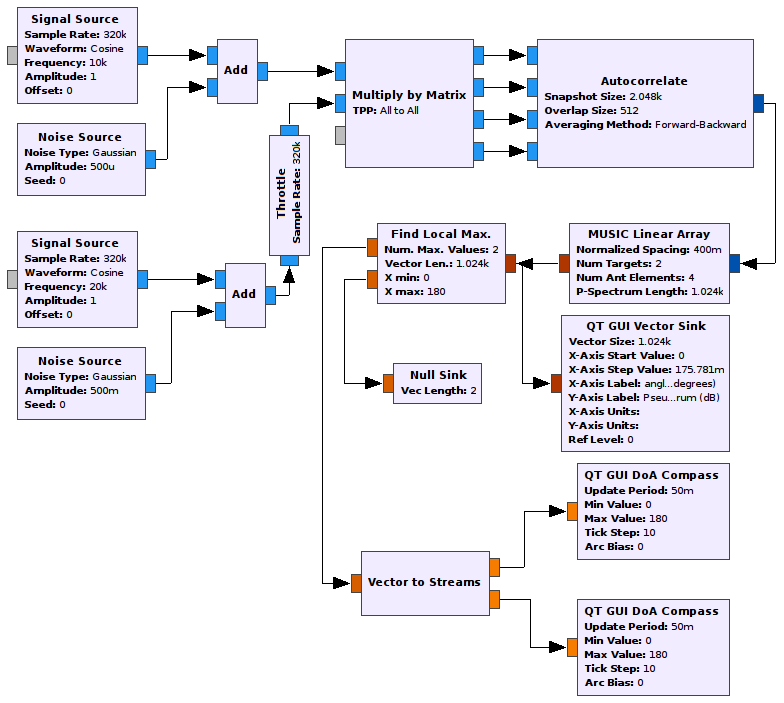
\includegraphics[width=\textwidth]{src/img/graph-doa}
    \caption{Lanțul de procesare din implementarea agloritmului MUSIC folosită}
    \label{fig:grc-fg}
\end{figure}

\section{Descrierea funcționalității}
\label{sec:gr-doa-desc}

\subsection{Pașii elementari ai algoritmului MUSIC}
\label{ssec:music-steps}

În Secțiunea \ref{sec:theory-music} s-a făcut o detaliere a algoritmului
MUSIC, împreună cu fundamentul matematic și demonstrațiile pe care se bazează.
În continuare, este util să identificăm pașii elementari ai algoritmului,
care se vor suprapune peste blocurile folosite în procesare. Reamintim faptul că
M reprezintă numărul de elemente ale șirului de antene și N este numărul de
semnale care ajung la fiecare dintre acestea. 

\subsection*{Pasul 1}
\label{sssec:step1}
Știind că semnalul $x_i$ ajunge la elementul cu numărul \textit{i} al șirului de
antene, matricea de autocorelație a intrării poate fi calculată astfel:
\begin{equation}
    \bm{R}_{xx} = E[\bm{xx}^H]
\end{equation}
\begin{equation}
    x = \begin{bmatrix}x_1 & x_2 & ... & x_M \end{bmatrix}
\end{equation}

\subsection*{Pasul 2}
\label{sssec:step2}
Estimarea numărului de semnale care ajung la fiecare element al șirului de
antene. Pentru a efectua acest pas, trebuie să calculăm valorile proprii ale
matricei $R_{xx}$ și, din ordinul de multiplicitate $K$ al celei mai mici valori
proprii, vom estima numărul de semnale astfel:
\begin{equation}
    \hat{N} = M - K
\end{equation}

\subsection*{Pasul 3}
\label{sssec:step3}
Calculăm spectrum spațial MUSIC folosindu-ne de Ecuația \eqref{eq:music-spatial-sp}.
\begin{equation}
    P_{MUSIC}(\theta) =
        \frac{\bm{a}^H(\theta)\bm{a}(\theta)}
             {\bm{a}^H(\theta)\bm{V}_N\bm{V}_N^H\bm{a}(\theta)} \\
\label{eq:music-spatial-sp}
\end{equation}
\begin{equation}
    \bm{V}_N = \begin{bmatrix}v_{N+1}, & ..., & v_M \end{bmatrix}
\end{equation}

\subsection*{Pasul 4}
\label{sssec:step4}
Căutăm maximele spectrului MUSIC estimat, care ne dau direcțiile de incidență
pentru cele $\hat{N}$ semnale.


\subsection{Descrierea blocurilor componente}
\label{ssec:gr-doa-desc-blocks}

Pentru a explica modul de lucru al lanțului de procesare, vom defini mai întâi o
serie de parametri folosiți în blocurile componente. Numele acestora nu reflectă
neapărat numele variabilelor folosite în cod, dar ne ajută să identificăm mai
bine noțiunile de interes.

\begin{itemize}
  \item \code{sample\_rate} Rata la care este eșantionat semnalul
  \item \code{tone\_freq\_i} Frecvența semnalului de pe intrarea $i$
  \item \code{norm\_spacing} Distanța normată dintre elementele șirului de
  antene
  \item \code{num\_targets} Numărul de semnale de intrare care ajung la șirul de
  antene, denumit în unele situații și N
  \item \code{num\_array\_elements} Numărul de elemente din șirul de antene,
  denumit în unele situații și M
  \item \code{spectrum\_length} Numărul de elemente al spectrului MUSIC calculat
  \item \code{snapshot\_size} Dimensiunea capturii, adică numărul de eșantioane
  folosite pentru calculul autocorelației, denumit și K
  \item \code{overlap\_size} Numărul de eșantioane care se suprapun la
  calcularea unor valori succesive ale autocorelației
\end{itemize}

Cu cât sistemul dispunde de un număr mai mare de antene, cu atât rezoluția
spațială obținută va fi mai bună, iar cu cât dimensiunea capturii pentru autocorelație
este mai mare, cu atât acuratețea detecției va crește, deoarece mai puține
eșantioane în calculul autocorelației se traduc într-o corelație estimată mai
puternică a semnalelor de intrare, lucru care nu este de dorit~\cite{oumar2012comparison}.

\subsection{Datele de intrare}
În configurația actuală, se folosesc două surse de semnal ($N = 2$) care
generează forme de undă cosinusoidale cu frecvențe de 10 kHz și 20 kHz, peste
care adăugăm zgomot Gaussian, și un șir de antene cu patru elemente ($M = 4$).
Blocul \textbf{Throttle} este folosit pentru a limita volumul de date la
frecvența semnalului de la intrare, așa cum s-ar comporta într-un caz real.
Nefolosirea acestui bloc ar presupune consumarea tuturor resurselor de procesare
disponibile pe dispozitivul de calcul. Particularizarea este făcută pentru a
facilita explicarea blocurilor componente și nu îngrădește în niciun fel
generalizarea ulterioară pentru un set diferit de parametri de intrare.

\subsection{Blocul ,,Multiply by Matrix''}
Acest bloc este folosit pentru a simula felul în care semnalele ajung la șirul
de antene, înmulțind matricea colectoare a șirului cu un vector format din
eșantioane ale semnalului de intrare. Dacă  $\bm{A}$ este matricea dată ca
parametru de intrare al blocului, de dimensiune $M \times N$, și
$\bm{X}_N$ este un vector coloană alcătuit din cele $N$ intrări ale blocului,
atunci rezultatul înmulțirii este:
\begin{equation}
\bm{Y}_M = \bm{A}\bm{X}_N,
\end{equation}
unde $\bm{Y}_M$ un vector coloană construit din ieșirile blocului. Prin urmare,
blocul trebuie să aibă un număr de N intrări și M ieșiri. \\

Matricea colectoare are în vedere unghiurile de incidență și distanța
normată dintre elementele șirului de antene. Distanța normată reprezintă
distanța dintre antene exprimată în metri împărțită la lungimea de undă a purtătoarei.
Conform~\cite{ettus-doa}, distanța normată trebuie să fie cel mult jumătate
din lungimea de undă a semnalului, deoarece, în caz contrar, ar apărea fenomenul
de aliere spectrală, care ar putea deteriora rezoluția algoritmului MUSIC. \\

În cazul nostru, matricea colectoare este
\begin{displaymath}
    A
    =
    \begin{bmatrix}
        \bm{a}(\theta_1) & \bm{a}(\theta_2)
    \end{bmatrix}
\end{displaymath}
unde $\bm{a}(\theta_i)$  este vectorul director corespunzător unghiului de
incidență $\theta$ al semnalului $i$. Ieșirile blocului \textbf{Multiply by Matrix}
reprezintă suma semnalelor care ajung sub diferite unghiuri de incidență la
fiecare antenă.

\subsection{Blocul ''Autocorrelate''}
\label{ssec:autocorrelate-block}
Următorul bloc, \textbf{Autocorrelate}, corespunde pasului \S1 al algoritmului
MUSIC, deși calculează, de fapt, un estimat al autocorelației semnalului sub
forma unei matrice de corelație eșantionată. O metodă de calcul a acestei
matrice este de a colecta un număr de K eșantioane într-o perioadă de timp
denumită ,,captură'', formând matricea $\bm{X_K}$ de dimensiune $N \times K$,
ceea ce conduce la următoarea formulă:
\begin{equation}
C_x = \frac{1}{K}\bm{X_K}\bm{X_K}^H.
\label{eq:autocorr-first-part}
\end{equation}

În~\cite{fb-averaging} s-a sugerat faptul că adăugarea unui pas de mediere
antegradă-retrogradă a matricei de corelație eșantionată va crește performanțele
estimării unghiului de incidență, astfel încât calculul se ajustează după cum
urmează:
\begin{equation}
C_x = \frac{1}{2K}\bm{X_K}\bm{X_K}^H + \frac{1}{2K}\bm{J}\bm{X_K}^*\bm{X_K}^T\bm{J},
\end{equation}
unde J este o matrice de reflexie (elementele diagonalei secundare sunt egale cu
1 și restul sunt egale cu 0). \\

Parametrii blocului \textbf{Autocorrelate} sunt:
\begin{itemize}
    \item Dimensiunea de captură, denumită K, ce reprezintă numărul de
    eșantioane de intrare folosite în calculul matricei de corelație pentru un
    element de ieșire.
    \item Dimensiunea de suprapunere, adică numărul de eșantioane care se
    suprapun în calculul a două matrice de corelație succesive.
    \item Metoda de mediere, care poate fi antegradă-retrogradă, retrogradă, sau metoda
    standard antegradă.
\end{itemize}

\subsection{Blocul ,,MUSIC Linear Array''}
\label{ssec:music-lin-array}
În această aplicație, presupunem cunoscut numărul de semnale de intrare, deci nu
avem nevoie de un bloc separat pentru pasul \S2. Prin urmare, trecem direct la
blocul \textbf{MUSIC Linear Array} care calculează spectrul MUSIC din pasul \S3.
\\

În constructorul blocului se formează un vector colector care cuprinde toate
unghiurile posibile dintr-o deschidere de 180 grade, cu o rezoluție de
\code{1/spectrum\_length}. Cu cât un unghi folosit în generarea vectorului
colector este mai aproape de unghiul de incidență, cu atât mai aproape va fi
spectrul MUSIC de 0. În teorie, când acestea coincid, spectrul MUSIC tinde la 0
când numărul de observații tinde la infinit. Prin urmare, pentru fiecare dată de
intrare, un număr de \code{spectrum\_length} valori ale spectrului MUSIC va
trebui calculat, din care va fi păstrată doar partea reală, deoarece ne
interesează doar amplitudinea spectrului MUSIC. \\

Pentru a calcula spectrul MUSIC, blocul primește ca intrare rezultatul
autocorelației, care este descompus apoi în vectori proprii, și spectrul este
calculat conform Formulei \eqref{eq:music-spectrum}. Blocul primește ca
parametri de intrare numărul de surse de semnal, numărul de antene, distanța
normată dintre ele și lungimea spectrului.

\subsection{Blocul ,,Find Local Max''}
Pentru ca aplicația să găsească valorile unghiurilor de incidență, este nevoie
de blocul \textbf{Find Local Max}, care realizează pasul \S4 al algoritmului.
Blocul oferă la ieșire unghiurile la care sunt găsite maximele din spectru și
caută exact $N$ astfel de maxime. El oferă, de asemenea, informații despre
amplitudinea maximelor, dar din moment ce ele nu sunt de interes pentru
aplicație sunt direcționate către un bloc denumit \textbf{Null Sink}, care le
înlătură.

\subsection{Vizualizarea rezultatelor}
\begin{figure}[h]
    \centering
    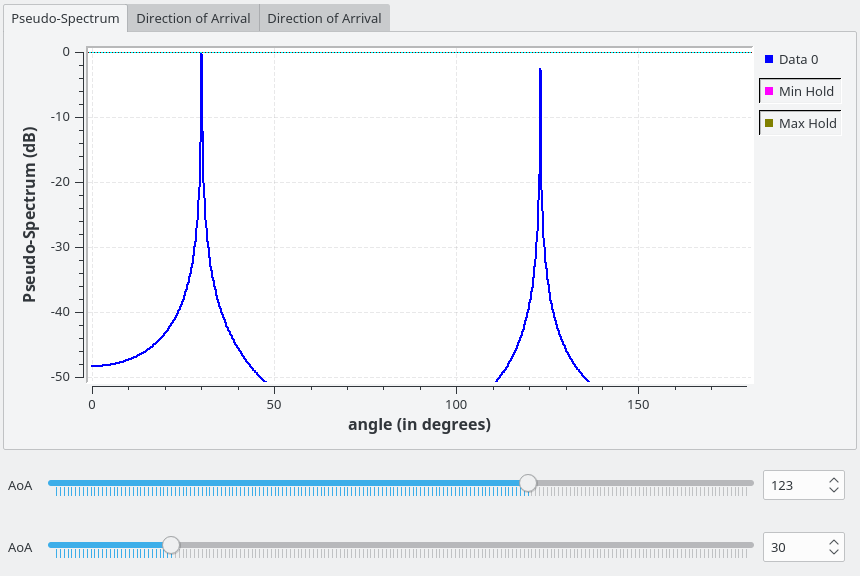
\includegraphics[width=0.75\textwidth]{src/img/grc-doa-spectrum}
    \caption{Spectrul MUSIC}
    \label{fig:doa-sp}
\end{figure}

Putem vizualiza spectrul fie imediat după blocul \textbf{MUSIC Linear
Array}, precum în Figura \ref{fig:doa-sp}, și să ne formăm o idee despre unghiul
de incidență măsurat cu blocul \textbf{QT GUI Vector Sink} sau, folosind blocul
\textbf{QT GUI DoA Compass}, putem vedea precis unghiul estimat pentru cele două
semnale după procesarea din blocul \textbf{Find Local Max}. Se poate observa un
exemplu de astfel de ieșire pentru unul dintre semnalele de intrare în Figura
\ref{fig:doa-compass}. Folosind două cursoare, putem schimba unghiurile de
incidență în timp real și să observăm cum algoritmul se adaptează acestor
schimbări. 

\begin{figure}[h]
    \centering
    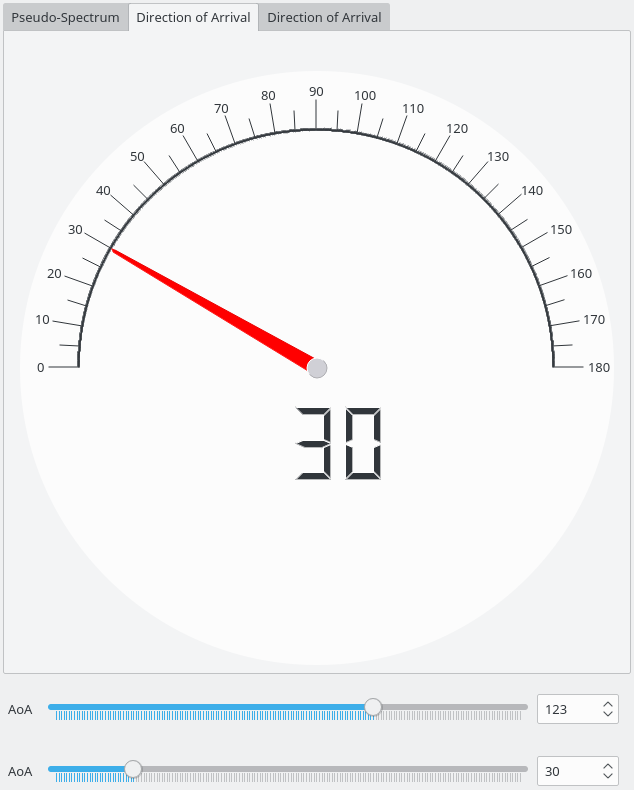
\includegraphics[width=0.4\textwidth]{src/img/grc-doa-compass}
    \caption{Unghiul de incidență estimat pentru unul dintre semnalele de intrare}
    \label{fig:doa-compass}
\end{figure}

\section{Evaluarea profilului de execuție al implementării algoritmului MUSIC}
\label{sec:gr-doa-perf}

Implementarea \code{gr-doa} folosește biblioteca Armadillo~\cite{arma}
pentru efectuarea operațiilor comune de algebră liniară în limbajul C++. Pentru
descompunerea matricelor folosește biblioteca LAPACK~\cite{lapack} (Linear Algebra PACKage),
care oferă rutine pentru rezolvarea sistemelor de ecuații liniare, probleme de
valori proprii și descompunerea valorilor singulare ale unei matrice. 
LAPACK se folosește de BLAS (Basic Linear
Algebra Subprograms)~\cite{blas}, o specificație care descrie un set de rutine
\textit{low-level} pentru operații algebrice precum adunări de vectori, produs
scalar, produs vectorial, combinații liniare și înmulțire de matrice. Există mai
multe implementări posibile ale specificației BLAS, care se folosesc, în
general, de instrucțiuni specifice sistemului folosit, precum suportul hardware
pentru operații în virgulă mobilă sau instrucțiuni SIMD, ajungând la performanțe
deosebite. Armadillo poate efectua înmulțiri de matrice și fără suportul BLAS,
dar acestea au o performanță redusă și anumite descompuneri de matrice pot
deveni indisponibile fără LAPACK și BLAS. În evaluarea performanțelor, ne-am
asigurat că \code{gr-doa} folosește LAPACK și BLAS pentru atingerea unor
performanțe maxime.

\subsection{Metodologia de evaluare}
\label{sec:met-eval-perf}
Interfața grafică GNU Radio Companion generează un script Python bazat pe lanțul
de procesare creat, care folosește apoi SWIG~\cite{swig}, un utilitar care
îi permite să acceseze codul C++ și să execute graful. Din cauza acestui pas
intermediar, performanțele evaluate pe baza scriptului nu sunt foarte relevante,
deoarece funcții folosite în procesul de interfațare a codului Python cu codul
C++ ajung să consume o mare parte din timpul de execuție. Din acest motiv,
soluția preferată a fost crearea unui program C++ care construiește lanțul de
procesare într-un mod similar, ceea ce elimină și dependența de o interfață
grafică. \\

În acest program am eliminat toate blocurile dependente de Qt și, unde a fost
necesar, le-am înlocuit cu blocuri \textbf{Null Sink}, care pur și simplu ignoră
datele primite, deci din acest punct de vedere nu avem operațiuni de I/O
consumatoare de timp. În plus, blocul \textbf{Throttle} a fost eliminat,
deoarece vrem să evaluăm programul atunci când este executat la viteză maximă,
fără constrângeri. \\

Există două variante de execuție a lanțului de procesare, în funcție de tipul de
surse de intrare folosite:
\begin{itemize}
  \item Dacă se folosesc blocuri care generează anumite tipuri de semnal de
  intrare și de zgomot, se consideră că lanțul de procesare are un număr infinit
  de date de intrare și execuția sa se va termina  dacă i se va
  încheia execuția în mod explicit după un anumit interval de timp.
  Dezavantajul, în acest caz, este faptul că generarea semnalelor consumă
  resurse de procesare importante, care pot introduce erori cu privire la profilul
  programului într-o situație reală în care am folosi antene fizice și semnalele de
  intrare nu ar trebui simulate. Din acest motiv, această variantă va fi
  folosită doar în testare.

  \item Dacă se folosesc blocuri care citesc semnalele de intrare din fișiere în
  care au fost salvate, în prealabil, eșantioane ale semnalelor dorite, se
  elimină procesarea nedorită din cazul anterior, deci vom folosi această
  variantă în generarea profilurilor de execuție. Execuția lanțului de procesare
  nu mai trebuie încheiată în mod explicit, deoarece acest lucru se va petrece
  automat, odată cu citirea tuturor datelor din fișierele sursă.
\end{itemize}

Pentru evaluarea profilului de execuție, am folosit
\textbf{perf\_events}~\cite{perf}, care realizează un \textit{profil} al unui
program în funcție de un eveniment dorit.  Perf\_events este un
utilitar foarte puternic pentru măsurarea unui set mare de evenimente hardware,
care permite examinarea codului de asamblare pentru funcțiile de interes, ceea
ce poate fi de ajutor atunci când se urmăresc micro-optimizări.  În acest caz,
am fost interesați de procentul din numărul total de cicli de execuție petrecut
în diferite funcții, pentru a distinge punctele critice din execuția programului
unde se pot aplica optimizări și care pot fi accelerate cu ajutorul procesorului
ConnexArray. \\

Perf\_events se bazează pe eșantionarea evenimentelor și o perioadă
este exprimată în termeni de evenimente petrecute, nu de perioade de tact. El se
folosește de numărătoare pe 64 biți emulate în software și colectează un
eșantion atunci când numărătorul se resetează. Acest eșantion este un termen
generic pentru un anumit tip de eveniment pentru care se realizează profilul. El
reține informații despre punctul în care era programul în momentul colectării
eșantionului, deci în momentul în care a fost întrerupt, sub forma unui
\textit{pointer la instrucțiune}. \\

\abbrev{PMU}{Performance Monitoring Unit}
În hardware, sistemele au implementate o unitate de monitorizare a performanței
(Performance Monitoring Unit - PMU), care colectează statistici despre
procesor și starea memoriei. Motivul pentru care perf\_events emulează un
numărător pe 64 biți este faptul că PMU nu pune la dispoziție un astfel de
registru hardware, iar acest lucru poate deveni important în momentul
în care se interpretează locația unde a avut loc o întrerupere în cazul unui
profil bazat pe eșantionarea întreruperilor, pentru că locul unde a avut loc o
întrerupere PMU poate diferi de locul unde s-a resetat numărătorul software. \\

În cazul de față, numărul de cicli petrecuți în funcțiile
programului se pot obține folosind \code{perf record}, ce folosește în mod
implicit ciclii ca tip de eveniment. Acest tip de eveniment generic este mapat
la o implementare hardware specifică de către PMU care, pentru procesoarele
Intel și sistemele AMD, nu menține o corelație constantă între eveniment și
timp, din cauza unei scalări în frecvență (evenimentul se numește, în acest caz,
\textit{unhalted}), ceea ce înseamnă că ciclii nu sunt numărați atunci când
procesorul nu lucrează (se află în starea \textit{idle}). Prin urmare, această
analiză ne oferă informații doar despre procesarea efectivă din anumite blocuri,
nu și despre timpul pe care acestea îl petrec, de exemplu, așteptând date de
intrare. Pentru un profil asupra acestui aspect se pot verifica evenimente
precum \textit{stalls} sau \textit{cache misses}. \\

Recapitulând, folosind \textbf{perf\_events}, putem obține informații despre
ciclii petrecuți în funcțiile programului folosind comanda din Listarea
\ref{lst:perf-command}, unde a fost specificat și tipul de eveniment ce se
dorește înregistrat prin argumentul \code{-e cycles}. În plus, am adăugat și
opțiunea \code{--call-graph dwarf}, care permite folosirea standardului de date
pentru \textit{debugging} DWARF pentru a obține informații despre \textit{call
stack} (stiva de apeluri).

\begin{lstlisting}[
  language=bash,
  caption={Comandă pentru profil realizat cu perf},
  label={lst:perf-command}
  ]
perf record -e cycles --call-graph dwarf ./run_MUSIC_profile

\end{lstlisting}

Pentru a obține rezultate corecte, este important ca programul să fie compilat
utilizând \textit{frame pointers} (pointeri la cadre), care sunt, în general,
omiși din motive de optimizare și fără de care este posibil să obținem un profil
incomplet. \\

Lanțul de procesare este executat folosind mai multe fire de execuție,
gestionate de GNU Radio, iar comanda de mai sus, folosită per proces, va agrega
statisticile pentru fire de execuție la nivelul procesului, această opțiune de
moștenire fiind activată în mod implicit.

\subsection{Rezultatele evaluării pe un procesor Intel Core i7-6500U}

Într-o primă etapă, performanțele implementării \code{gr-doa} au fost evaluate
pe un procesor Intel Core i7-6500U, cu frecvența de \SI{2,50}{GHz} pentru a
identifica punctele cheie din execuție care pot fi optimizate. \\

Folosind nivelul minim de optimizare și activând simbolurile de
\textit{debugging}, cele mai importante rezultate (pentru funcțiile care consumă
mai mult de 2\% din numărul total de cicli) sunt prezentate în Tabelul
\ref{tab:prof-o3}.

%=============================================================================
% Profiling table
%=============================================================================
\begin{table}[!htb]
\begin{center}
 \begin{tabular}{||c c c||} 
 \hline
 Overhead  & Command & Symbol \\ [0.5ex] 
 \hline\hline
 49,14\% 
 &
 find\_local\_max6
 &
 \makecell{arma::glue\_hist::apply\_noalias<unsigned int>}
 \\ 
 
 \hline
 13,73\%
 &
 autocorrelate4
 &
 \makecell{cgemm\_}
 \\
 
  \hline
 10,51\%
 &
 MUSIC\_lin\_array
 &
 \makecell{cgemm\_}
 \\
 
 \hline
 3,63\%
 &
 multiply\_matrix
 &
 \makecell{\_\_mulsc3}
 \\

  \hline
 3,56\%
 &
 MUSIC\_lin\_array
 &
 \makecell{cgemv\_}
 \\

  \hline
 3,06\%
 &
 MUSIC\_lin\_array
 &
 \makecell{gr::doa::MUSIC\_lin\_array\_impl::work}
 \\

  \hline
 2,33\%
 &
 MUSIC\_lin\_array
 &
 \makecell{\_\_logf\_finite}
 \\

  \hline
 2,08\%
 &
 multiply\_matrix  
 &
 \makecell{gr::blocks::multiply\_matrix\_cc\_impl::work}
 \\ [1ex] 
 \hline
\end{tabular}
\end{center}
\caption{Profilul lanțului de procesare MUSIC realizat pe un procesor Intel Core
i7}\label{tab:prof-o3}
\end{table}


Conform documentației~\cite{perf-doc}, \textit{Overhead} este procentul din
numărul total de cicli petrecuți într-o anumită funcție, \textit{Command} este
numele \textit{task}-ului care poate fi citit cu \code{/proc/<pid>/comm}, și
\textit{Symbol} este numele funcției aflate în execuție la momentul sondării. \\

Investigând în continuare, am aflat că se petrece cel mai mult timp în funcția
\code{arma::} \code{glue\_hist::apply\_noalias<unsigned int>}, din biblioteca
\textbf{Armadillo}, care este apelată din funcția \code{find\_local\_max} și care
se ocupă de găsirea maximelor din spectrul MUSIC. \\ 

Acest bloc poate fi implementat mai eficient, având în vedere că partea
intensivă din punct de vedere computațional poate fi evitată în majoritatea
cazurilor în care niciunul dintre punctele de maxim nu este egal $-\infty$. \\

Prin eliminarea acestei procesări acolo unde nu este necesară, obținem noile
rezultate de performanță în Tabelul \ref{tab:prof-remove}, unde au fost
prezentate doar funcțiile care consumă mai mult de 5\% din numărul total de
cicli de execuție. O vizualizare mai intuitivă asupra acestor rezultate este
oferită în Figura \ref{fig:profile-flamegraph}, realizată cu ajutorul
programului FlameGraph~\cite{flamegraph}. Acesta construiește un grafic pe baza
rezultatelor generate folosind perf\_events, cu următoarea interpretare:

\begin{itemize}
  \item Fiecare bloc reprezintă o funcție (\textit{stack frame}).
  \item Pe axa verticală se află adâncimea stivei, adică ordinea de apelare a
  funcțiilor (,,descendenți'') din interiorul altor funcții (care reprezintă
  ,,părinții'' acestora). Blocul care reprezintă funcția părinte se află
  întotdeauna sub blocul care reprezintă funcția descendent, deci funcția
  rădăcină se află pe nivelul cel mai de jos al graficului, iar funcția frunză
  pe cel mai înalt.
  \item Lățimea blocurilor este direct proporțională cu frecvența cu care au
  apărut în raporturile de activitate a stivei (\textit{stack traces}).
\end{itemize}

%=============================================================================
% Profiling table
%=============================================================================
\begin{table}[H]
\begin{center}
 \begin{tabular}{||c c c||} 
 \hline
 Overhead  & Command & Symbol \\ [0.5ex] 
 \hline\hline
 28,63\% 
 &
 autocorrelate9
 &
 \makecell{cgemm\_}
 \\ 
 
 \hline
 23,16\%
 &
 MUSIC\_lin\_array
 &
 \makecell{cgemm\_}
 \\
 
 \hline
 5,40\%  
 &
 multiply\_matrix
 &
 \makecell{\_\_mulsc3}

 \\
 
 \hline
 5,04\%  
 &
 autocorrelate9
 &
 \makecell{std::conj<float>}
 \\ [1ex] 
 \hline
\end{tabular}
\end{center}
\caption{Profilul lanțului de procesare MUSIC realizat pe un procesor Intel
Core i7 după aplicarea corecțiilor în algoritmul de identificare a maximelor
spectrului MUSIC}\label{tab:prof-remove} 
\end{table}


\begin{figure}[h]
    \centering
    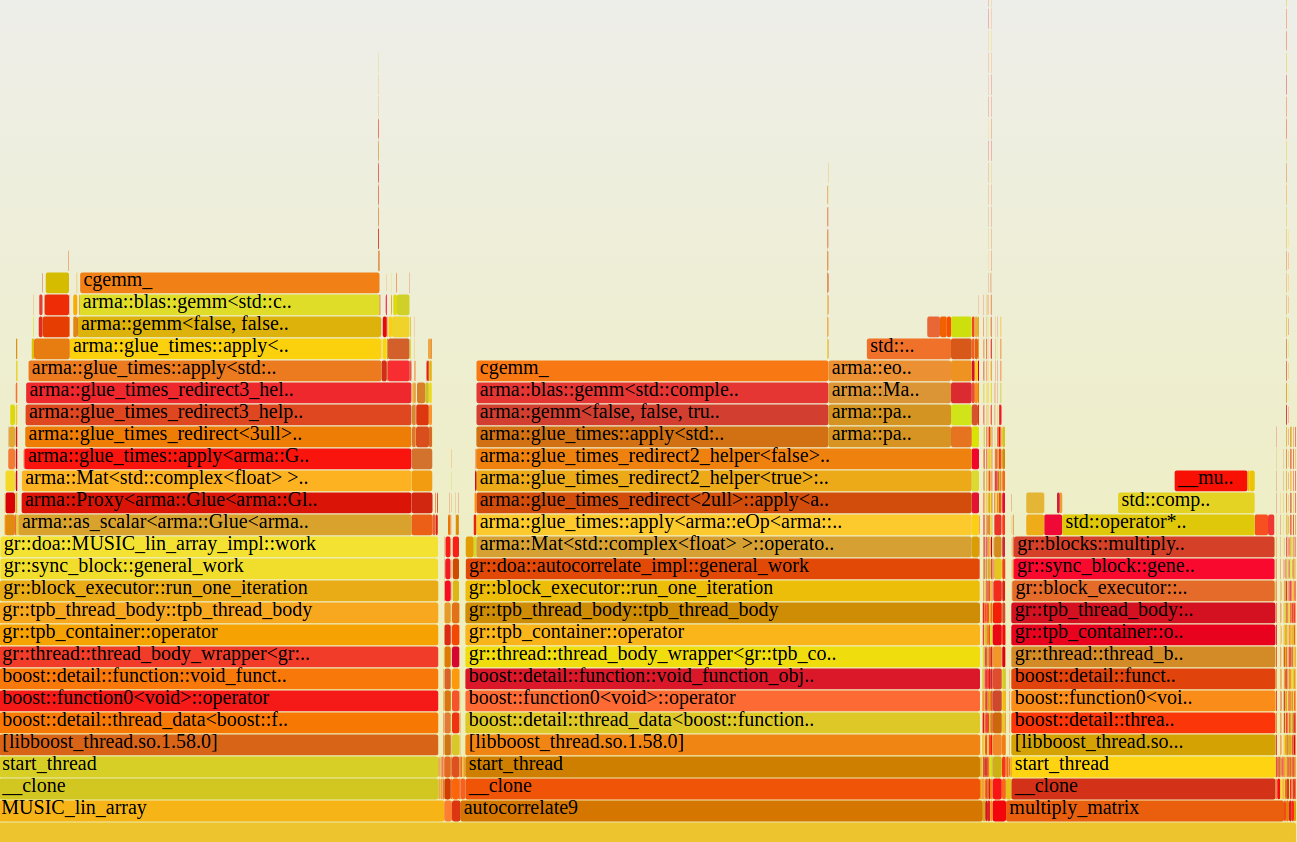
\includegraphics[width=1\textwidth]{src/img/flamegraph-orig-fs}
    \caption{Vizualizarea profilului de execuție pe un procesor Intel Core i7 cu ajutorul FlameGraph}
    \label{fig:profile-flamegraph}
\end{figure}

Observăm, în primul rând, că cele mai importante blocuri din punct de vedere al
procesării sunt \textbf{Autocorrelate} și \textbf{MUSIC Linear Array}, detaliate
în Secțiunile \ref{ssec:autocorrelate-block}, și, respectiv,
\ref{ssec:music-lin-array}. Al treilea rezultat, \textbf{Multiply by Matrix} nu
prezintă relevanță din punct de vedere practic deoarece scopul lui este doar să
simuleze un semnal care vine dintr-o anumită direcție. Ultimul rezultat din
tabel reprezintă operația de conjugare a unui număr complex, apelată din blocul
de autocorelație. \\

În al doilea rând, observăm că operațiile cu simbolul \code{cgemm\_} consumă o
parte importantă din resursele de procesare, ele fiind responsabile de
înmulțirile de matrice definite în biblioteca BLAS.  Cu ajutorul perf\_events,
putem să vedem exact în ce părți din cod se apelează funcții care au nevoie de
această rutină. \\

\lstset{
	language=C++,
	directivestyle={\color{black}},
	emph={int,char,double,float,unsigned},
	emphstyle={\color{RoyalBlue}}
    }		
\begin{lstlisting}[
	firstnumber=105,
	caption={Punctul critic din funcția de autocorelație},
	label={lst:hot-autocorrelation}
    ]
out_matrix =
    (1.0 / d_snapshot_size) * d_input_matrix.st() * conj(d_input_matrix);
\end{lstlisting}

În privința blocului care realizează autocorelația, punctul critic este în
calculul efectiv al estimatului autocorelației corespunzător Formulei
\eqref{eq:autocorr-first-part}. Listarea \ref{lst:hot-autocorrelation} prezintă
partea din cod care realizează acest calcul. Matricea
\code{d\_input\_matrix} este formată din cele \code{snapshot\_size} eșantioane
ale semnalului de intrare folosit în calculul autocorelației, care ajung la cele
\newline
\code{num\_array\_elements} antene. Acesta este stocat deja în forma sa
transpusă, ceea ce explică diferența dintre formulă și implementarea din cod.
Punctul cheie în această parte este faptul că dimensiunea capturii este, în
general, un număr mare (de exemplu, 2048), deoarece dorim să asigurăm o estimare
cât mai fidelă, deci și matricele care se înmulțesc vor avea un număr mare de
elemente. \\

În ceea ce privește blocul \textbf{MUSIC Linear Array}, punctul în care se
apelează rutina pentru înmulțirile de matrice se află în calculul
spectrului MUSIC folosind Formula \eqref{eq:music-spectrum}. Partea din cod care
efectuează acest calcul se găsește la linia 136, în Listarea
\ref{lst:hot-music}. În această porțiune de cod, matricea \code{d\_vii\_matrix}
conține pe fiecare coloană vectorii directori, iar matricea
\code{d\_vii\_matrix\_trans} este transpusa și conjugata acesteia. Matricea
\code{U\_N\_sq} este obținută din produsul $\bm{V}_N\bm{V}_N^H$, unde $\bm{V}_N$
este format din vectorii proprii ai matricei de covarianță care sunt
perpendiculari pe subspațiul semnalelor. \\

Este important, în acest caz, faptul că matricea \code{d\_vii\_matrix} este
calculată o singură dată, în constructorul blocului, iar fiecare coloană din
acest vector este înmulțită cu aceeași matrice calculată pe baza intrării
blocului. Avem, așadar, un număr egal cu dimensiunea spectrului MUSIC de
înmulțiri înlănțuite dintre un vector linie, o matrice și un vector coloană a
căror dimensiune depinde de numărul de antene din sistem, deci numărul total de
înmulțiri va fi relativ mare în comparație cu dimensiunea tablourilor care se
înmulțesc. \\

\lstset{
	language=C++,
	directivestyle={\color{black}},
	emph={int,char,double,float,unsigned},
	emphstyle={\color{RoyalBlue}}
    }		
\begin{lstlisting}[
	firstnumber=134,
	caption={Punctul critic din blocul MUSIC Linear Array},
	label={lst:hot-music}
    ]
for (int ii = 0; ii < d_pspectrum_len; ii++)
{
  Q_temp = 
    as_scalar(d_vii_matrix_trans.row(ii) * U_N_sq * d_vii_matrix.col(ii));
  out_vec(ii) = 1.0 / Q_temp.real();
}
\end{lstlisting}

\subsection{Rezultatele evaluării pe placa de dezvoltare Xilinx
ZedBoard Zynq-7000 \mbox{ARM/FPGA} SoC}

Am evaluat performanțele și pe placa de dezvoltare Zedboard Zynq-7000, prezentată
în Secțiunea~\ref{sec:cnx-arr}, și am ajuns la concluzia că procentajele obținute
sunt asemnănătoare. \\

Tabela \ref{tab:prof-zedboard} prezintă rezultatele care consumă mai mult de 5\%
din timpul total de procesare al evaluării pe procesorul Dual-Core ARM Cortex
A9, realizată în aceeași configurație ca și cea de pe procesorul Intel.

%=============================================================================
% Profiling table
%=============================================================================
\begin{table}[H]
\begin{center}
 \begin{tabular}{||c c c||} 
 \hline
 Overhead  & Command & Symbol \\ [0.5ex] 
 \hline\hline
 18,97\% 
 &
 autocorrelate9
 &
 \makecell{cgemm\_}
 \\ 
 
 \hline
 13,68\%
 &
 MUSIC\_lin\_array
 &
 \makecell{cgemm\_}
 \\
 
 \hline
 5,93\%  
 &
 autocorrelate9
 &
 \makecell{gr::doa::autocorrelate\_impl::general\_work}
 \\
 
 \hline
 5,79\%  
 &
 MUSIC\_lin\_array
 &
 \makecell{cgemv\_}
 \\
 
 \hline
 5,76\%  
 &
 MUSIC\_lin\_array
 &
 \makecell{gr::doa::MUSIC\_lin\_array\_impl::work}
 \\ [1ex] 
 \hline
\end{tabular}
\end{center}
\caption{
Profilul lanțului de procesare MUSIC realizat pe un procesor ARM Cortex A9 după
aplicarea corecțiilor în algoritmul de identificare a maximelor spectrului
MUSIC}
\label{tab:prof-zedboard}
\end{table}


\section{Testare}
\label{sec:testing}

Testarea întregului lanț de procesare este o etapă esențială nu numai pentru
determinarea corectitudinii rezultatelor finale, dar și pentru evaluarea
preciziei obținute. Conceptul de \textit{unit testing} este o metodă utilă în
acest scop, cu care se pot testa blocuri individuale sau agregate ale unui
produs software, fiind un instrument indispensabil în industria
software. \\

Deși GNU Radio are încorporate metode pentru testarea blocurilor dezvoltate, nu
oferea suficientă flexibilitate pentru a putea fi utilizate în testarea folosind
simulatorul sau suportul hardware a kernelurilor de accelerare într-o
etapă viitoare, motiv pentru care a trebuit să recurgem la altă soluție.
Biblioteca \textbf{Google Test}~\cite{gtest} s-a dovedit a fi o soluție mai bună
în acest sens, testele putând fi scrise cu ușurință și executate cu ajutorul
unui script care pornește simulatorul, atunci când este cazul, și prin
intermediul căruia pot fi oferite căile pentru cozile de comunicare cu
acceleratorul ca argumente în linia de comandă către program. \\

În Google Test se definesc \textit{aserțiuni}, adică afirmații a căror valoare
de adevăr trebuie stabilită. Aceste aserțiuni sunt folosite de teste pentru a
verifica comportamentul codului: dacă rezultatele obținute sunt diferite de cele
așteptate sau dacă se întâlnește altă eroare în timpul execuției codului, un
test eșuează, iar în caz contrar se consideră trecut. Testele pot fi grupate în
\textit{test case}-uri, iar un program de test poate să cuprindă mai multe
astfel de \textit{test case}-uri. \\

Lanțul de procesare are nevoie de o serie de parametri prezentați în Secțiunea 
\ref{ssec:gr-doa-desc-blocks}, la care se vor adăuga cozile prin care se va
comunica cu procesorul ConnexArray și, eventual, alți parametri cu care să putem
controla forma de undă a semnalului de intrare sau tipul de zgomot care se
adaugă peste acesta. Definim o clasă \code{flowgraph\_parameters} care are ca
date membre acești parametri de intrare și metode pentru setarea valorilor
acestora. O altă clasă, \code{doa\_flowgraph}, are un membru de tip
\code{flowgraph\_parameters} și o metodă prin care construiește un
\textit{flowgraph} cu parametrii primiți prin intermediul acesteia. În Anexa
\ref{sec:test-header} se găsește codul sursă al fișierului header care conține
declarațiile claselor menționate. \\

Metoda care construiește lanțul de procesare folosit în testare este similară cu
cea descrisă în Secțiunea \ref{sec:met-eval-perf} pentru evaluarea
performanțelor, cu excepția faptului că datele de ieșire nu mai sunt ignorate,
ci direcționate către un bloc care le va returna la ieșire, pentru a fi preluate
de către testele definite și apoi verificate. Codul care implementează
construcția \textit{flowgraph}-ului pentru două semnale de intrare se găsește în
Anexa \ref{sec:test-code}. \\

În Listarea \ref{lst:test-example} este prezentat un exemplu de definire a unui
test, în care mai întâi se construiește o instanță a clasei de parametri cu
datele dorite, care este apoi folosită pentru a crea clasa responsabilă de
lanțul de procesare. Se folosește tipul de aserțiune \code{EXPECT\_THAT}, care
compară valorile unghiurilor de incidență găsite cu cele specificate în
parametrii de intrare, cu o anumită eroare a cărei valoare poate fi controlată.
De exemplu, dacă sursele au unghiuri de incidență foarte apropiate, dacă
unghiul de incidență se află la limitele domeniului, sau dacă raportul
semnal-zgomot este foarte mic, ne putem aștepta la o precizie mai redusă. \\

Am definit mai multe clase de teste care verifică acuratețea rezultatelor în
următoarele situații:
\begin{itemize}
  \item Sursele provin din unghiuri relativ distante, caz în care precizia ar
  trebui să fie foarte bună, cu o eroare de mai puțin de $\varepsilon = 0.2^{\circ}$.
  \item Direcțiile de incidență ale celor două surse sunt foarte apropiate
  (între $10^{\circ}$ și $2^{\circ}$) sau se află la limitele intervalului de
  $[0^{\circ}, 180^{\circ}]$, caz în care precizia scade cu până la $\varepsilon =
  1^{\circ}$ în cazurile extreme.
  \item Frecvențele semnalelor sunt foarte apropiate, dar în acest caz nu s-au
  observat modificări de precizie semnificative, cel puțin în simulări.
  \item Diferite dimensiuni ale spectrului MUSIC, care modifică rezoluția
  obținută, deci afectează și precizia.
  \item Diferite dimensiuni ale capturii pe care se calculează autocorelația,
  cu același efect asupra preciziei.
  \item Diferite configurații de antene.
\end{itemize}

\lstset{
    language=C++,
    directivestyle={\color{black}},
    emph={int,char,double,float,unsigned},
    emphstyle={\color{RoyalBlue}}
}
\begin{lstlisting}[
    caption={Exemplu de test realizat cu Google Test},
    label={lst:test-example}
]
TEST(DoaTwoSourcesTest, GeneralTest) {
    auto fg_params = flowgraph_parameters<2>()
                        .set_sample_rate(320000)
                        .set_norm_spacing(0.4)
                        .set_num_array_elements(4)
                        .set_p_spectrum_length(1024)
                        .set_snapshot_size(2048)
                        .set_overlap_size(512)
                        .set_nr_output_items(1024)
                        .set_freq({10000, 20000})
                        .set_theta_deg({40, 120})
                        .set_signal_amplitude({1, 1})
                        .set_noise_amplitude({0.005, 0.00005})
                        .set_waveform({gr::analog::GR_COS_WAVE,
                                       gr::analog::GR_COS_WAVE})
                        .set_noise_type({gr::analog::GR_GAUSSIAN,
                                         gr::analog::GR_GAUSSIAN})
                        .set_distributionFIFO(my_argv[1])
                        .set_reductionFIFO(my_argv[2])
                        .set_writeFIFO(my_argv[3])
                        .set_readFIFO(my_argv[4]);
    auto doa_fg = doa_flowgraph<2>(fg_params);
    EXPECT_THAT(doa_fg.build_flowgraph(), UnorderedElementsAre(
                        FN_HIGH_PRECISION(40),
                        FN_HIGH_PRECISION(120)));
}
\end{lstlisting}



\section{Concluzii}
\label{sec:impl-concl}

Având în vedere rezultatele obținute, putem concluziona că punctele critice în
procesarea algoritmului MUSIC au loc la înmulțirile de tablouri unidimensionale
sau bidimensionale de numere complexe, fie că este vorba de înmulțirea dintre un
vector și conjugatul său, ca în cazul autocorelației, fie că vorbim de
înmulțirea dintre un vector și o matrice, sau de un produs înlănțuit dintre un
vector, o matrice și un alt vector. Așadar, merită să ne îndreptăm atenția
spre implementarea unor kerneluri pentru procesorul ConnexArray care să
efectueze aceste operații, care vor fi detaliate în Capitolul
\ref{chapter:acc}, urmând a le evalua performanțele în Capitolul
\ref{chapter:eval}. \\

Așa cum a fost subliniat la începutul Secțiunii \ref{sec:gr-doa-perf},
înmulțirile dintre tablouri de date sunt efectuate utilizând implementări ale
specificației BLAS, cu suport în implementarea hardware a sistemului pe care se lucrează.
Ele exploatează ierarhia memoriei unui sistem, localizarea datelor (\textit{data
locality}), împărțind datele pe care se operează în blocuri care sunt
transferate în memoria de pe diferite niveluri. Cu cât un tip de memorie este
mai rapidă, cu atât ea dispune de un spațiu de stocare mai mic; o clasificare a
memoriilor în funcție de viteză, începând de la cea mai rapidă, este următoarea:
registre, cache (care poate fi, la rândul său, împărțit pe mai multe niveluri),
memoria principală, memoria secundară (\textit{disk}). Dacă tablourile de date
pe care se operează au dimensiuni foarte mari, ele nu vor putea fi aduse în
intregime în cea mai rapidă memorie și de aceea este necesar să se opereze pe
blocuri de date care să circule între tipurile de memorii enumerate, caz în care
transferul I/O va consuma mai mult timp de execuție. \\

Având în vedere acest raționament, putem presupune că în implementarea
kernelurilor vom avea un avantaj suplimentar atunci când dimensiunile matricelor
vor fi mai mari, comparativ cu implementarea BLAS. Chiar și când acesta nu va fi
cazul, vom încerca să efectuăm mai multe înmulțiri simultan, pentru un grad mai
mare de paralelizare. \\

Un alt aspect interesant este și faptul că în anumite situații se poate exploata
și dimensiunea tablourilor de date, astfel că, de exemplu, biblioteca
OpenBLAS~\cite{openblas} conține instrucțiuni specifice pentru diferite tipuri de
procesoare care iau în calcul și dimensiunea matricelor pentru un plus de
performanță~\cite{openblas-repo}. Prin urmare, acolo unde este cazul, vom lua în considerare
adaptarea algoritmilor la anumite dimensiuni ale unor matrice pentru a le crește
performanța. \\

Referitor la întregul ansamblu de procesare care implementează algoritmul MUSIC,
trebuie menționat faptul că este posibil ca optimizarea unui singur bloc poate
fi ,,mascată'' în evaluarea performanțelor de existența altui bloc mai lent,
care va încetini întregul lanț de procesare. Cu alte cuvinte, blocurile sunt
dependente unul de celălalt prin schimbul de date care are loc între ele și, în
cazul în care un bloc reprezintă un \textit{bottleneck}, performanțele
întregului lanț de procesare vor avea de suferit din această cauză.




